\section{Results: distortion}
\label{sec:distortion}

\emph{The exact second moment.} Distortion is measured on all rows of each data set, scaled to $[0, 1]$ on all rows (classification scales on the training rows only). Equation~\eqref{eq:variance} was checked over \N{vm:draws} draws on 2,000 pairs per data set in all \N{vm:cells} cells. The measured variance of $q$ is within about \N{vm:max_dev_pct}\% of the formula in every cell (about \N{vm:k3_dev_pct}\% for $k \ge 3$), and the mean of $q$ lies between \N{vm:mean_q_min} and \N{vm:mean_q_max}. The study's own 100 draws are too few at small $k$: the ratio of measured to predicted variance runs from \N{vm100:ratio_min} to \N{vm100:ratio_max}. So Eq.~3's $q$ has a lower variance than the Gaussian's, Eq.~4's the same, and matrices with $s > 3$ a higher one, as the theory says.

\emph{Equal variance is not equal distortion.} On Iris at $k = 2$, Eq.~4 preserves rank and neighbors worse than the Gaussian: the Spearman correlation of distances is \N{dz:iris:2:eq4:spearman_mean} (over the draws whose projection is not all zero) against \N{dz:iris:2:gauss:spearman_mean}, and the 5-nearest-neighbor label agreement is \N{dz:iris:2:eq4:knn5_agreement_mean} against \N{dz:iris:2:gauss:knn5_agreement_mean} (\N{dz:iris:2:gauss:knn5_agreement_original_mean} with all features).

\emph{The tail bound is loose.} The per-pair tail bound of Dasgupta and Gupta, which holds for Gaussian matrices, is never exceeded here by the share of pairs averaged over draws, for any family or cell, and except for one nonzero per column, it is far from tight (on Breast Cancer at $k = 24$, one nonzero per column has \N{dz:breast_cancer:24:opc:share_low_05_mean}\% of pairs at $q \le 0.5$ against a bound of \N{dz:breast_cancer:24:opc:bound_low_05}\%). On Breast Cancer at $k = 2$ (Fig.~\ref{fig:tails}), \N{dz:breast_cancer:2:gauss:share_low_05_mean}\% of pairs shrink to half their squared distance or less for the Gaussian, against an exact \N{dz:breast_cancer:2:gauss:gauss_exact_low_05}\% and a bound of \N{dz:breast_cancer:2:gauss:bound_low_05}\%.

\begin{figure}[t]
\centering
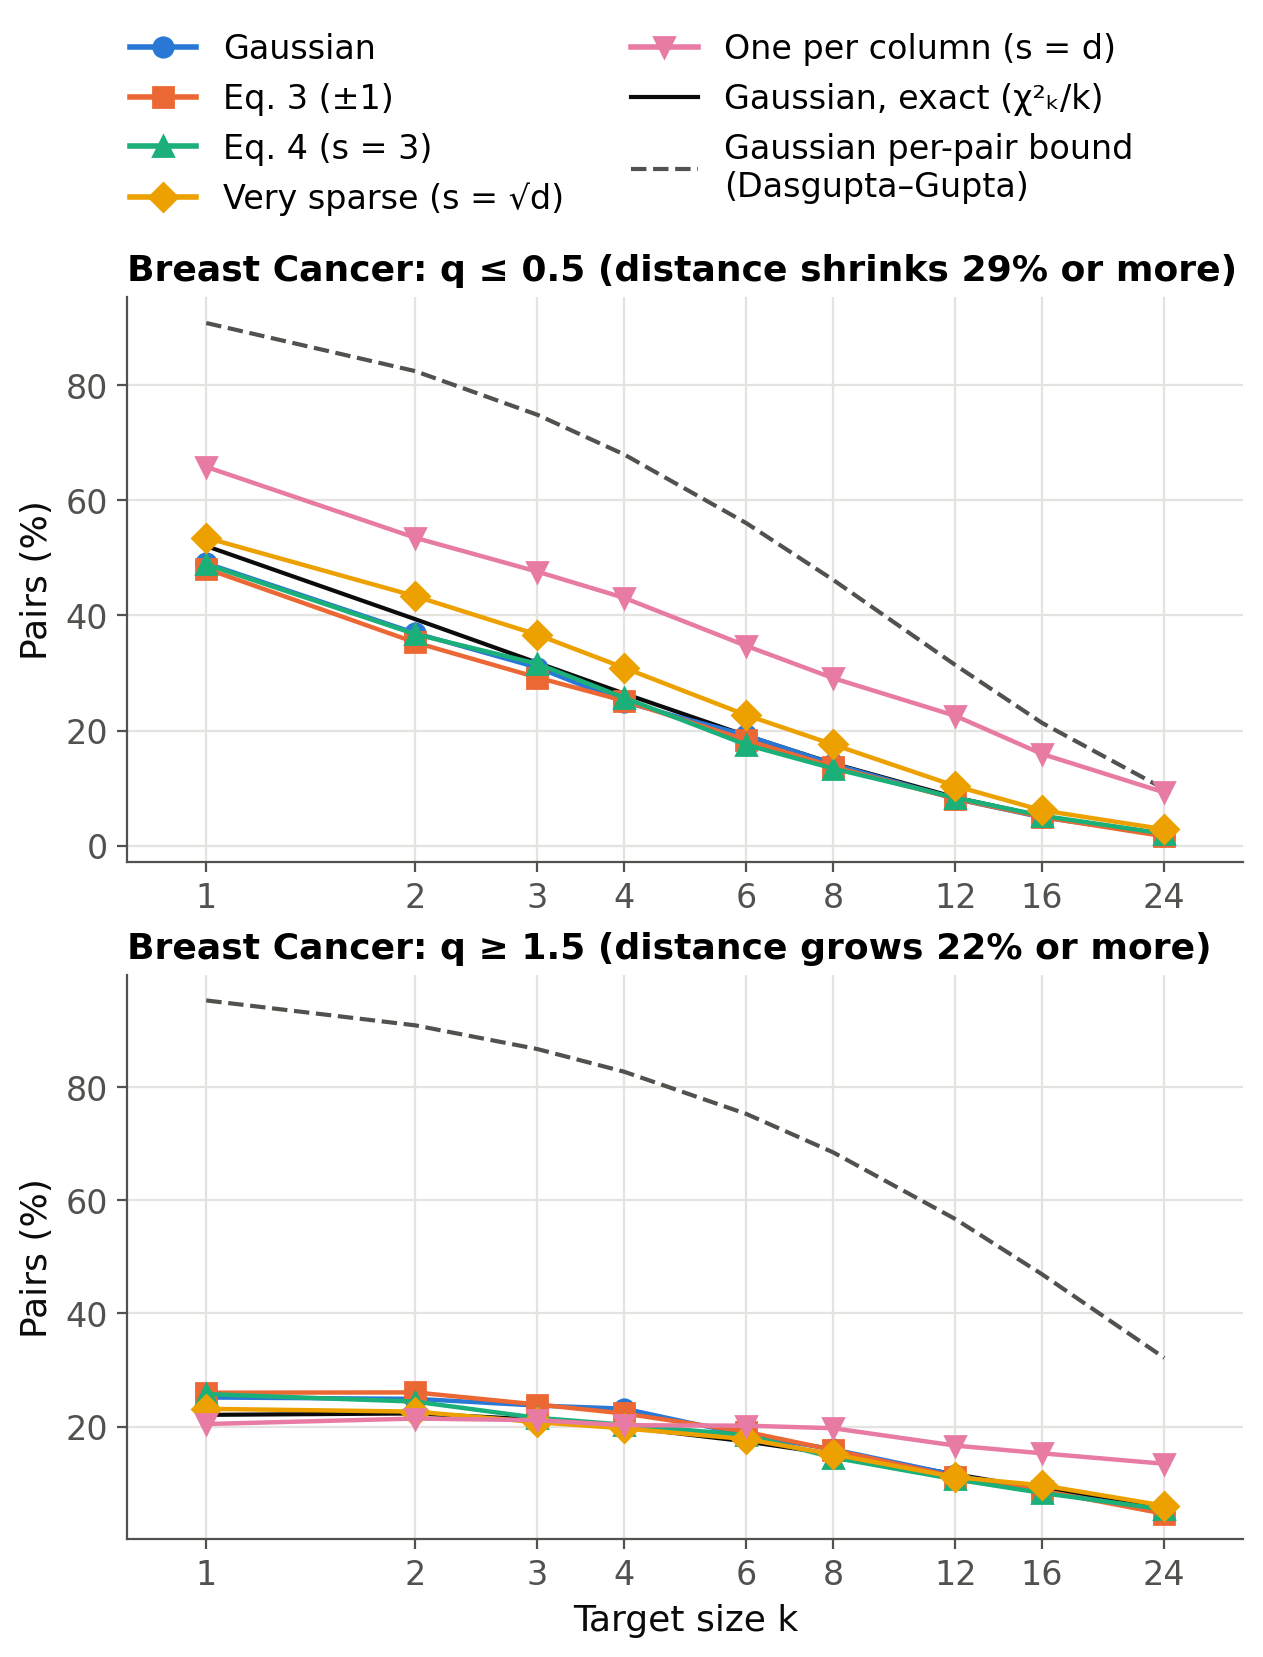
\includegraphics[width=\columnwidth]{../study/figures/fig4_distortion_tails_vs_bound.png}
\caption{Share of Breast Cancer pairs with $q \le 0.5$ (top) and $q \ge 1.5$ (bottom) against target size $k$, for each family, with the Gaussian's exact law and per-pair bound.}
\label{fig:tails}
\end{figure}

\emph{Variance does not explain accuracy.} Read as a heuristic, not a theorem, the variance order suggests that Eq.~3 should be at least as accurate as the Gaussian. It is not: Eq.~3 minus Gaussian is negative in \N{c:eq3_neg} of \N{c:eq3_cells} cells, pooled \N{pool:eq3:gauss} points. Within a data set and a fixed $k$, model-free neighbor agreement after projection does track accuracy across families (not shown), but no experiment here manipulates it, so it is a correlation and not a cause.
